\documentclass[11pt,a4paper]{article}

\typeout{------------------------------------------------------------------}
\typeout{} 
\typeout{        Fichier de base modifie par : Matth: 20 nov 2012} 
\typeout{                   sous licence GNU-GPL} 
\typeout{}
\typeout{------------------------------------------------------------------}

% Classe générale du document
   %documentclass[12pt,a4paper]{article} % .10pt, 11pt, 12pt : taille de la police principale (10 par défaut)
                 % .a4paper, letterpaper,... : délimite la taille du papier. (letterpaper par défaut)
	         % .fleqn : aligne les formules mathématiques à gauche au lieu de les centrer.
		 % .leqno : place la numérotation des formules à gauche plutôt qu'à droite.
		 % .twocolumn : demande à LATEX de formater le texte sur deux colonnes.
		 % .twoside, oneside indique si la sortie se fera en recto-verso ou en recto simple.
		 % .landscape, mais il faut mettre en commentaire (ou modifier) toutes les dimmensions

% Importation de packages divers
%   \NeedsTeXFormat{LaTeX2e} 
   \usepackage[T1]{fontenc}
   \usepackage[utf8x]{inputenc}		% utilisation des caractères 8 bits en Unix (codage ISO 8859-1)
  %\usepackage[latin1]{inputenc}	% utilisation des caractères pour Linux2
   \usepackage[usenames]{color}
   \usepackage{fancyhdr}
   \usepackage{lastpage}                % pour l'affichage du n° de la dernière page.
   \usepackage{lmodern}
   \usepackage{multirow}                % pour l'utilisation de figures ``noyées'' dans le texte
   \usepackage{xspace}			% package pour babel
   \usepackage[english]{babel}         % Utilisation du français (nom des sections, césure, ponctuation,...)
   \usepackage[english]{varioref}        % vpageref
   \usepackage{amsmath,amsthm,amssymb}  % Utilisation de certains packages de AMS (cf. belles équations)
   \usepackage{endnotes}                % Pour l'utilisation des notes en fin de documents
   \usepackage{verbatim}                % Pour l'insertion de fichier en mode verbatim
   \usepackage{portland}		% pour l'utilisation de \portrait et de \landscape sur une page
   \usepackage[pdftex]{graphicx}        % [pdftex] si utilisation d'images jgp,...
                                        % [dvips]  si utilisation d'images bmp,...
   \usepackage{pdfpages}		% Inclure des pages de pdf
   \usepackage{pdflscape}		% rotate => begin{landscape} ... \end{landscape}
   \usepackage{setspace}		% Pour définir un interligne
   \usepackage{tkz-orm}
   \usepackage[bottom]{footmisc}        % Footnote at the bottom
%   \usepackage[cyr]{aeguill}		% Pour les guillemets à la Française
   \usepackage{eurosym}			% Pour les Euro
   \usepackage{url}
    \urlstyle{sf}
   \usepackage[backgroundcolor=yellow]{todonotes} %% todonotes: \listoftodos & \todo{Some note or other.} & \missingfigure{}
	
   \renewcommand{\contentsname}{Sommaire} % si tableofcontents au début
   \newcommand{\Numero}{\No}
   \newcommand{\numero}{\no}
%   \newcommand{\fup}[1]{\up{#1}}

   \DeclareGraphicsExtensions{.jpg,.pdf,.mps,.png}       % déclaration d'extensions  pour les images
   %\input xy                            % pour le package xy (construction de diagramme)
   %\xyoption{all}

% Dimensions de la page :       	

  %%%%%%%%%%%%%%%%%%%%%%%%%%%%%%%%%%%%%%%%  0
  %   |                                  %
  %---+----------------------------------%  1
  %   | +----------------------------+   %  2
  %   | |          en-tête           |   %
  %   | +----------------------------+   %  3
  %   | +----------------------------+   %  4
  %   | |                            |   %       Remarques : 
  %   | |                            |   %        . distance de '0' à '1' : un pouce + \voffset
  %   | |                            |   %        . distance de 'a' à 'b' : un pouce + \hoffset
  %   | |           texte            |   %
  %   | |                            |   %
  %   | |                            |   %
  %   | |                            |   %
  %   | +----------------------------+   %  5
  %   | +----------------------------+   %
  %   | |         bas de page        |   %
  %   | +----------------------------+   %  6
  %%%%%%%%%%%%%%%%%%%%%%%%%%%%%%%%%%%%%%%%
  %a  b c                            d  e

%    % général
%      \voffset       0mm    % pour descendre (si positif) ou remonter (si négatif) le tout
%      \hoffset       0mm    % pour agrandir (si positif) ou diminuer (si négatif) la marge gauche (distance 'a' 'b')
%      \oddsidemargin 0mm   % 5pt  % distance de 'b' à 'c'
%     \evensidemargin 25mm  % 15pt % distance de 'd' à 'e'
%    % texte
%      \headsep       25pt   % distance de '3' à '4', la distance entre l'en-tête et le texte
%     \textheight    220mm  % distance de '4' à '5', pour déterminer la hauteur du texte
%     \textwidth     160mm  % distance de 'c' à 'd' 
%    % en-tête
%     \topmargin     0pt    % distance de '1' à '2', pour descendre (si positif) ou remonter (si négatif) le tout
%     \headheight    15pt   % distance de '2' à '3', doit être > 14.49999
%    % bas de page
%     \footskip      15mm   % 30pt % distance de '5' à '6', la distance entre le texte et le bas de page
     % space for the footnode
%    \setlength{\skip\footins}{1cm}

\usepackage[top=2.5cm, bottom=2.5cm, left=2.5cm, right=2.5cm]{geometry}

% (Re)définitions diverses

  % redéfinition de l'affichage des titres de section dans l'en-tête ou le bas de page
    % remarques :
    %  .affichage du numéro (2)    : \thesection 
    %  .affichage du nom (Section) : \sectionname
   % \renewcommand{\sectionmark}[1]{\markright{\thesection.\ #1}}   % 2.2. nom de la section 2.2
   % \renewcommand{\thesection}{\arabic{section}}		% II nom de la section 0.2


  % des couleurs...                   (utilisation avec par ex. \textcolor{webdarkblue}{...})
   \definecolor{codeBlue}{rgb}{0,0,1}
   \definecolor{webred}{rgb}{0.5,0,0}
   \definecolor{codeGreen}{rgb}{0,0.5,0}
   \definecolor{codeGrey}{rgb}{0.6,0.6,0.6}
   \definecolor{webdarkblue}{rgb}{0,0,0.4}
   \definecolor{webgreen}{rgb}{0,0.3,0}
   \definecolor{webblue}{rgb}{0,0,0.8}
   \definecolor{orange}{rgb}{0.7,0.1,0.1}

  % utilisation de caption, label,... pour autre chose qu'une figure
        %%%% debut macro %%%%
   \makeatletter
   \def\captionof#1#2{{\def\@captype{#1}#2}}
   \makeatother
        %%%% fin macro %%%%


% remarques : 
%  . pour mettre la date                  : \today
%  . pour mettre le nom de la section     : \rightmark
%  . pour mettre le numéro de page        : \thepage
%  . pour mettre le nombre de pages total : \pageref{LastPage}  (mais l'écrit en rouge vu que c'est une réf.)
%  . insertion d'une image                : \setlength{\unitlength}{1mm}
%                                             \begin{picture}(0,0)
%                                                \put(5,0){\includegraphics[scale=x.x]{xxx.xxx}}
%                                             \end{picture}

% Pour les guillemets à  la Française
\newcommand{\fermerguillemets}{\unskip\kern.15em\symbol{20}}
\newcommand{\ouvrerguillemets}{\symbol{19}\ignorespaces\kern.15em}
% \let »=\fermerguillemets
% \let« =\ouvrerguillemets

% Pour changer l'icone des puces : à placer juste avant une liste
 %   \renewcommand\labelitemi{\textbullet}	% Style boulet :)
\usepackage[pdfusetitle,
	    colorlinks=true,
	    linkcolor=webdarkblue, 
	    filecolor=webblue, 
	    urlcolor=webdarkblue,
	    citecolor=webgreen]{hyperref}     % pour l'utilisation des liens http,...

% Police
   %\renewcommand\familydefault{ptm}        % famille normale: Times ptm
   %\renewcommand\rmdefault{phv}            % famille à utiliser pour du Roman (phv)
   \renewcommand{\familydefault}{\sfdefault}

% L'interligne
%   \onehalfspacing % un et demi (= \setstrech{1.5} ou = \renewcommand{\baselinestretch}{1.5})
%   \renewcommand{\baselinestretch}{1.15}

     
% Mise en page
%   \pagestyle{fancy} %% custom en-tête
%   \usepackage[Matth]{fncychap}

% En-tete
%   \lhead{\texttt{LECGE1321} - Travail de Management Humain}        \chead{}        \rhead{Groupe 74}
%   \renewcommand{\headrulewidth}{0.5pt}     % pour l'épaisseur de la ligne

% Bas de page
%   \renewcommand{\footrulewidth}{0.5pt}       % pour l'épaisseur de la ligne
%   \lfoot{Partie \rightmark}        \cfoot{}        \rfoot{Page \thepage~sur~\pageref*{LastPageModif}}

% TOC jusqu'au subsection
\setcounter{tocdepth}{2} % Dans la table des matieres
\setcounter{secnumdepth}{3} % Avec un numero.

\usepackage{listings}
\lstset{
    language=Ruby,
	breakatwhitespace=true,
	breaklines=true,
	keepspaces=true,
	numbers=left,
	numbersep=5pt,
	showstringspaces=true,
	frame=single,
	basicstyle=\footnotesize,
	title=\lstname,
    literate=
      {á}{{\'a}}1 {é}{{\'e}}1 {í}{{\'i}}1 {ó}{{\'o}}1 {ú}{{\'u}}1
      {Á}{{\'A}}1 {É}{{\'E}}1 {Í}{{\'I}}1 {Ó}{{\'O}}1 {Ú}{{\'U}}1
      {à}{{\`a}}1 {è}{{\'e}}1 {ì}{{\`i}}1 {ò}{{\`o}}1 {ò}{{\`u}}1
      {À}{{\`A}}1 {È}{{\'E}}1 {Ì}{{\`I}}1 {Ò}{{\`O}}1 {Ò}{{\`U}}1
      {ä}{{\"a}}1 {ë}{{\"e}}1 {ï}{{\"i}}1 {ö}{{\"o}}1 {ü}{{\"u}}1
      {Ä}{{\"A}}1 {Ë}{{\"E}}1 {Ï}{{\"I}}1 {Ö}{{\"O}}1 {Ü}{{\"U}}1
      {â}{{\^a}}1 {ê}{{\^e}}1 {î}{{\^i}}1 {ô}{{\^o}}1 {û}{{\^u}}1
      {Â}{{\^A}}1 {Ê}{{\^E}}1 {Î}{{\^I}}1 {Ô}{{\^O}}1 {Û}{{\^U}}1
      {œ}{{\oe}}1 {Œ}{{\OE}}1 {æ}{{\ae}}1 {Æ}{{\AE}}1 {ß}{{\ss}}1
      {ç}{{\c c}}1 {Ç}{{\c C}}1 {ø}{{\o}}1 {å}{{\r a}}1 {Å}{{\r A}}1
      {€}{{\EUR}}1 {£}{{\pounds}}1
}

% Juste pour avoir un titre dans le pdf
\title{Software Development Project - Report 3}
\author{Group 6: Matthieu Baerts, Benoît Baufays, Julien Colmonts, Benjamin Frantzen, Pierre-Yves Légéna, Vincent Van Ouytsel, Ludovic Vannoorenberghe, Alex Vermeylen}

\begin{document}
\begin{titlepage}
\newgeometry{left=2cm,right=2cm,top=2cm,bottom=2cm}

\rm %% style Roman for the title

\begin{center}

% Upper part of the page
%\vspace*{-2cm}

\includegraphics[scale=.5]{ingi.png}\\[2cm]

\textsc{\LARGE Pôle d'ingénierie informatique}\\[1.5cm]

\textsc{\Large \texttt{LSINF2255} - Software Development Project}\\[0.5cm]


% Title
\vspace{3.5cm}
{ \huge \bfseries Requirements analysis report\vspace{0.8cm}}

\vspace{3.5cm}

% Author and supervisor
\begin{minipage}{0.4\textwidth}
\begin{flushleft} \large
\emph{Professor:}\\
	Kim \textsc{Mens}\\
\vspace{1cm}
\emph{Assistant:}\\
	Sergio \textsc{Castro Mejia} % Apple lover
\end{flushleft}
\end{minipage}
\begin{minipage}{0.4\textwidth}
\begin{flushright} \large
\emph{Students: (Group 6 - SINF2MS)} \\
%\begin{tabular}{rr}
	Matthieu \textsc{Baerts}\\
	Benoît \textsc{Baufays}\\
	(\textit{Project Manager}) Julien \textsc{Colmonts}\\
	Benjamin \textsc{Frantzen}\\
	Pierre-Yves \textsc{Légéna}\\
	Vincent \textsc{Van Ouytsel}\\
	Ludovic \textsc{Vannoorenberghe}\\
	Alex \textsc{Vermeylen}
%\end{tabular} \\
\end{flushright}
\end{minipage}

\vfill

% Bottom of the page
{\large Academic Year 2013-2014}
\end{center}

\end{titlepage}
\restoregeometry

\tableofcontents
%\thispagestyle{empty}	% pour enlever le numéro de page
\newpage
%\pagenumbering{arabic} % on triche avec la numéroation des pages :)

\section*{Introduction}
\addcontentsline{toc}{section}{Introduction}
At the begining of this phase, we just received the feedback of the previous one, so we knew the pros and cons of our work.
Looking at these informations, we decided to improve ourselves by taking the remarks in account.
The goals of this part of the job was to go further in the modelisation of the architecture of the program.
To do this, we had to create some diagrams : 
\begin{itemize}
\item A class diagram, showing the differents objects, their attributes, their main methods and the relations linking them.
\item Some sequences diagrams, to illustrate the most important user activities by displaying the interactions between the objects in several defined scenarios.
\item An ORM diagram, to show graphically the fields of the database and its architecture.
\item A box pointer diagram, to explain the way that the modules of the website are working together sequentially on a timeline.
\end{itemize}
Doing all theses diagrams will allow us to have a better overview of the project. So we will have a more precise idea on how the website will run. 
Two others requiered elements in this report were to detail the physical architecture and the framework that we chose and to argue the choice.
We had to do research to justify our choice and have a look on the physical architecture and how the chosen framework imposes it.

\newpage

\section{My title}
%\subsection{Application} %% TODO: another title...

\subsubsection{Class Diagram} %% TODO: another title...
See figure \vref{fig:uml}.\\
The class diagram shows the main classes of the model. Each variable of the class are detailled but only the main specific function that should be implemented are there and to avoid an overloading of the diagram we didn't list all the getters and setters of the variables. The hollow arrow shows the extended classes. For example, the classes Client and CoWorker extend User. The simple arrow shows a link between two classes and the indexes the number of this object that can be own by the class. When we see the link between address and user, it means that a user can have many addresses. But an organisation can have only one address.\\
Looking at the diagram we can see some classes extending user. There is client, coworker and moderator (extended by admin). This is due to the fact that there are all users but with specific rights on the website. Their is also the explicit link showing that a coworker of an organisation manage multiple client profiles. On another side, we have the moderator that are linked with the services categories. Another interesting part of the diagram is the architecture of the offer and demand. Each of these two objects are extending the "Service" abstract class and are linked with a transaction. The transaction is the conclusion of a matching. Service is an absctract class because we will never instantiate it directly.


\subsubsection{Sequences Diagrams} %% TODO: another title...

See figure \vref{fig:acceptService}.\\
See figure \vref{fig:addService}.\\
See figure \vref{fig:createUser}.\\
See figure \vref{fig:search}.\\
See figure \vref{fig:serviceFinished}.

\subsection{Physical Architectural View}



%– A physical architectural view of your software which describes how the logical architectural view is mapped to the physical components and connectors on your implementation platform (for example, different processors and other devices)
\begin{figure}[!ht]
	\begin{center}
		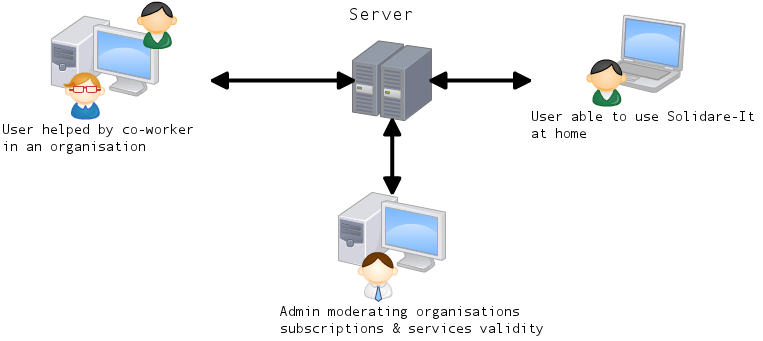
\includegraphics[width=\textwidth]{architectural_view_1.png}
		\caption{Website use}
		\label{fig:server}
	\end{center}
\end{figure}



\subsection{Pattern}
%– If applicable, a particular architectural style or pattern that is used. For example, it may be the case that the chosen web application framework imposes the use of a certain architectural pattern or architectural style (such as the model-view-controller architecture or MVC).

Ruby on Rails forces us to use the Model-View-Controller architectural style. Moreover, we all have experience with the MVC, then we will be more comfortable to code with this architecture.
\newpage

\newpage
\section*{Conclusion}
\addcontentsline{toc}{section}{Conclusion}
This work was the occasion to learn on one hand about software technology and on the other to improve our working organisation in a larger team than usual.
On this phase, our leader took his job very seriously by organizing and leading in meetings.
We also are more efficient with our collaborative development tools Trello and writeLatex.\\

We improve our experience of separating the work that has to be done in different parts.
We had to give back a consistent report so communication between us becomes really important.
To reach the goal before the deadline, we had to separate the job in different tasks attributed to subgroups.
In these subgroups working on different diagrams, we can still create responsibilities like two persons drawing the diagram on a white board and the third one transcript it into virtual file usable on the computer.\\

Now that we have a better module decomposition, we have a view on the time required to achieve this project.
The module decomposition allows us to improve the separation of the responsibilities. We hope that we gave you a better look on the project.
We have now a clear idea on what the application will be.
On development part, we have already thought about the minimal requirements of this architecture and we have also some ideas in our pockets to push the application .


%%We learn to DO NOT put exclamation mark in a technical document!


% \label{LastPageModif}

\newpage

\appendix
\pagenumbering{roman}
% \begin{landscape}

% \section{Appendix}

%\begin{figure}[!ht]
%	\begin{center}
%		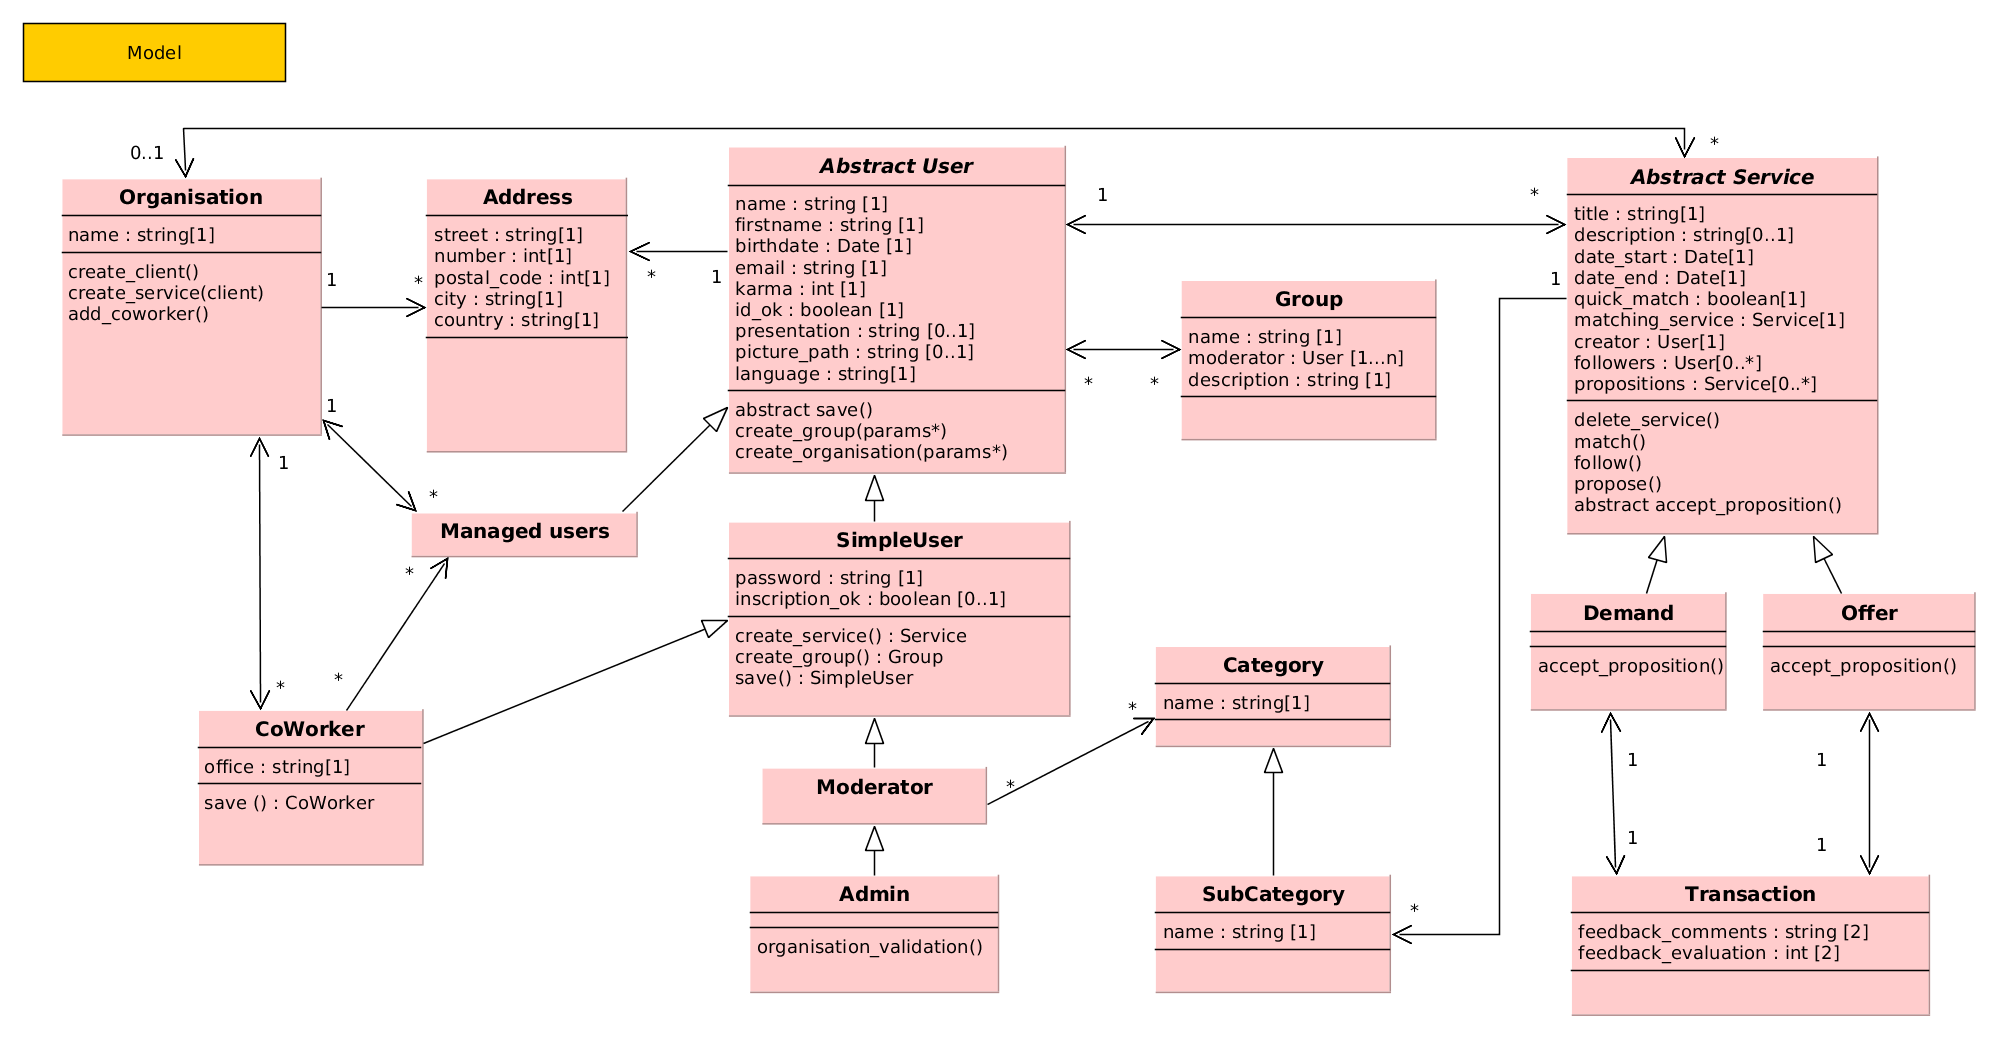
\includegraphics[width=.80\paperheight]{UML.png}
%		\caption{Unified Modeling Language (UML): class diagram}
%		\label{fig:uml}
%	\end{center}
%\end{figure}

% \end{landscape}



\end{document}
